\section{Coding}
\label{sec:Coding}

In this section, we will include the programming aspects of our design. All code is available in the GitHub repository at \url{https://github.com/grgao/boat/tree/main}. 

\subsection{Electromagnetic Coil Modeling and Range Calculations}
A critical component of the ASV's system is the electromagnetic coil, which generates a low-frequency magnetic field for underwater detection and tracking. To optimize the coil design and predict its performance, a Python-based simulation was developed. This code calculates the electrical properties of a rectangular coil and simulates the resulting magnetic moment, which is then used to calculate an effective range. 

The script first defines the coil geometry and material parameters, such as the number of turns, loop dimensions, wire size, and frequency. The inductance of the rectangular loop is calculated with a standard formula that accounts for  the loop's physical dimensions and number of turns. The resistance is determined from the total wire length and resistivity, while the impedance is computed at the operating frequency. The magnetic moment, which sets the strength of the magnetic field, is also calculated as $m = NIA$.

Once the magnetic moment of the coil is determined, the effective range is estimated using a model provided by Professor Strachen. We must first make some assumptions about the model. We model the coil as a magnetic dipole, and we assume that the underwater AUV has a field strength threshold of 2 nT, which is a reasonable value that the AUV teams were aiming for. The effective range is then calculated using the formula:

\begin{equation}
r = \left( \frac{\mu_0 m}{2 \pi B_r} e^{-\alpha r} \right)^{1/3}
\end{equation}
\begin{equation}
\alpha_s = \sqrt{\pi \cdot f \cdot \mu \cdot \sigma_W}
\end{equation}

where:
\begin{itemize}
    \item \( \mu_0 \) is the permeability of free space,
    \item \( m \) is the magnetic moment of the coil,
    \item \( B_r \) is the field strength threshold,
    \item \( \alpha \) is the attenuation coefficient given by the skin effect,
    \item \( f \) is the frequency of the signal,
    \item \( \mu \) is the permeability of the medium,
    \item \( \sigma_W \) is the conductivity of water, \SI{4 }{\siemens \per \meter}.
\end{itemize}

The effective range of different magnetic moments can be seen by Figure~\ref{fig:Effective Range}. With our magnetic moment of 59, we have an effective range of around 30 meters. The reason for a skin depth coefficient is due to the skin effect, which is a phenomenon where the current density decreases closer to the wires surface. This results in the magnetic field decaying exponentially with distance. 
\begin{figure}[H]
    \centering
    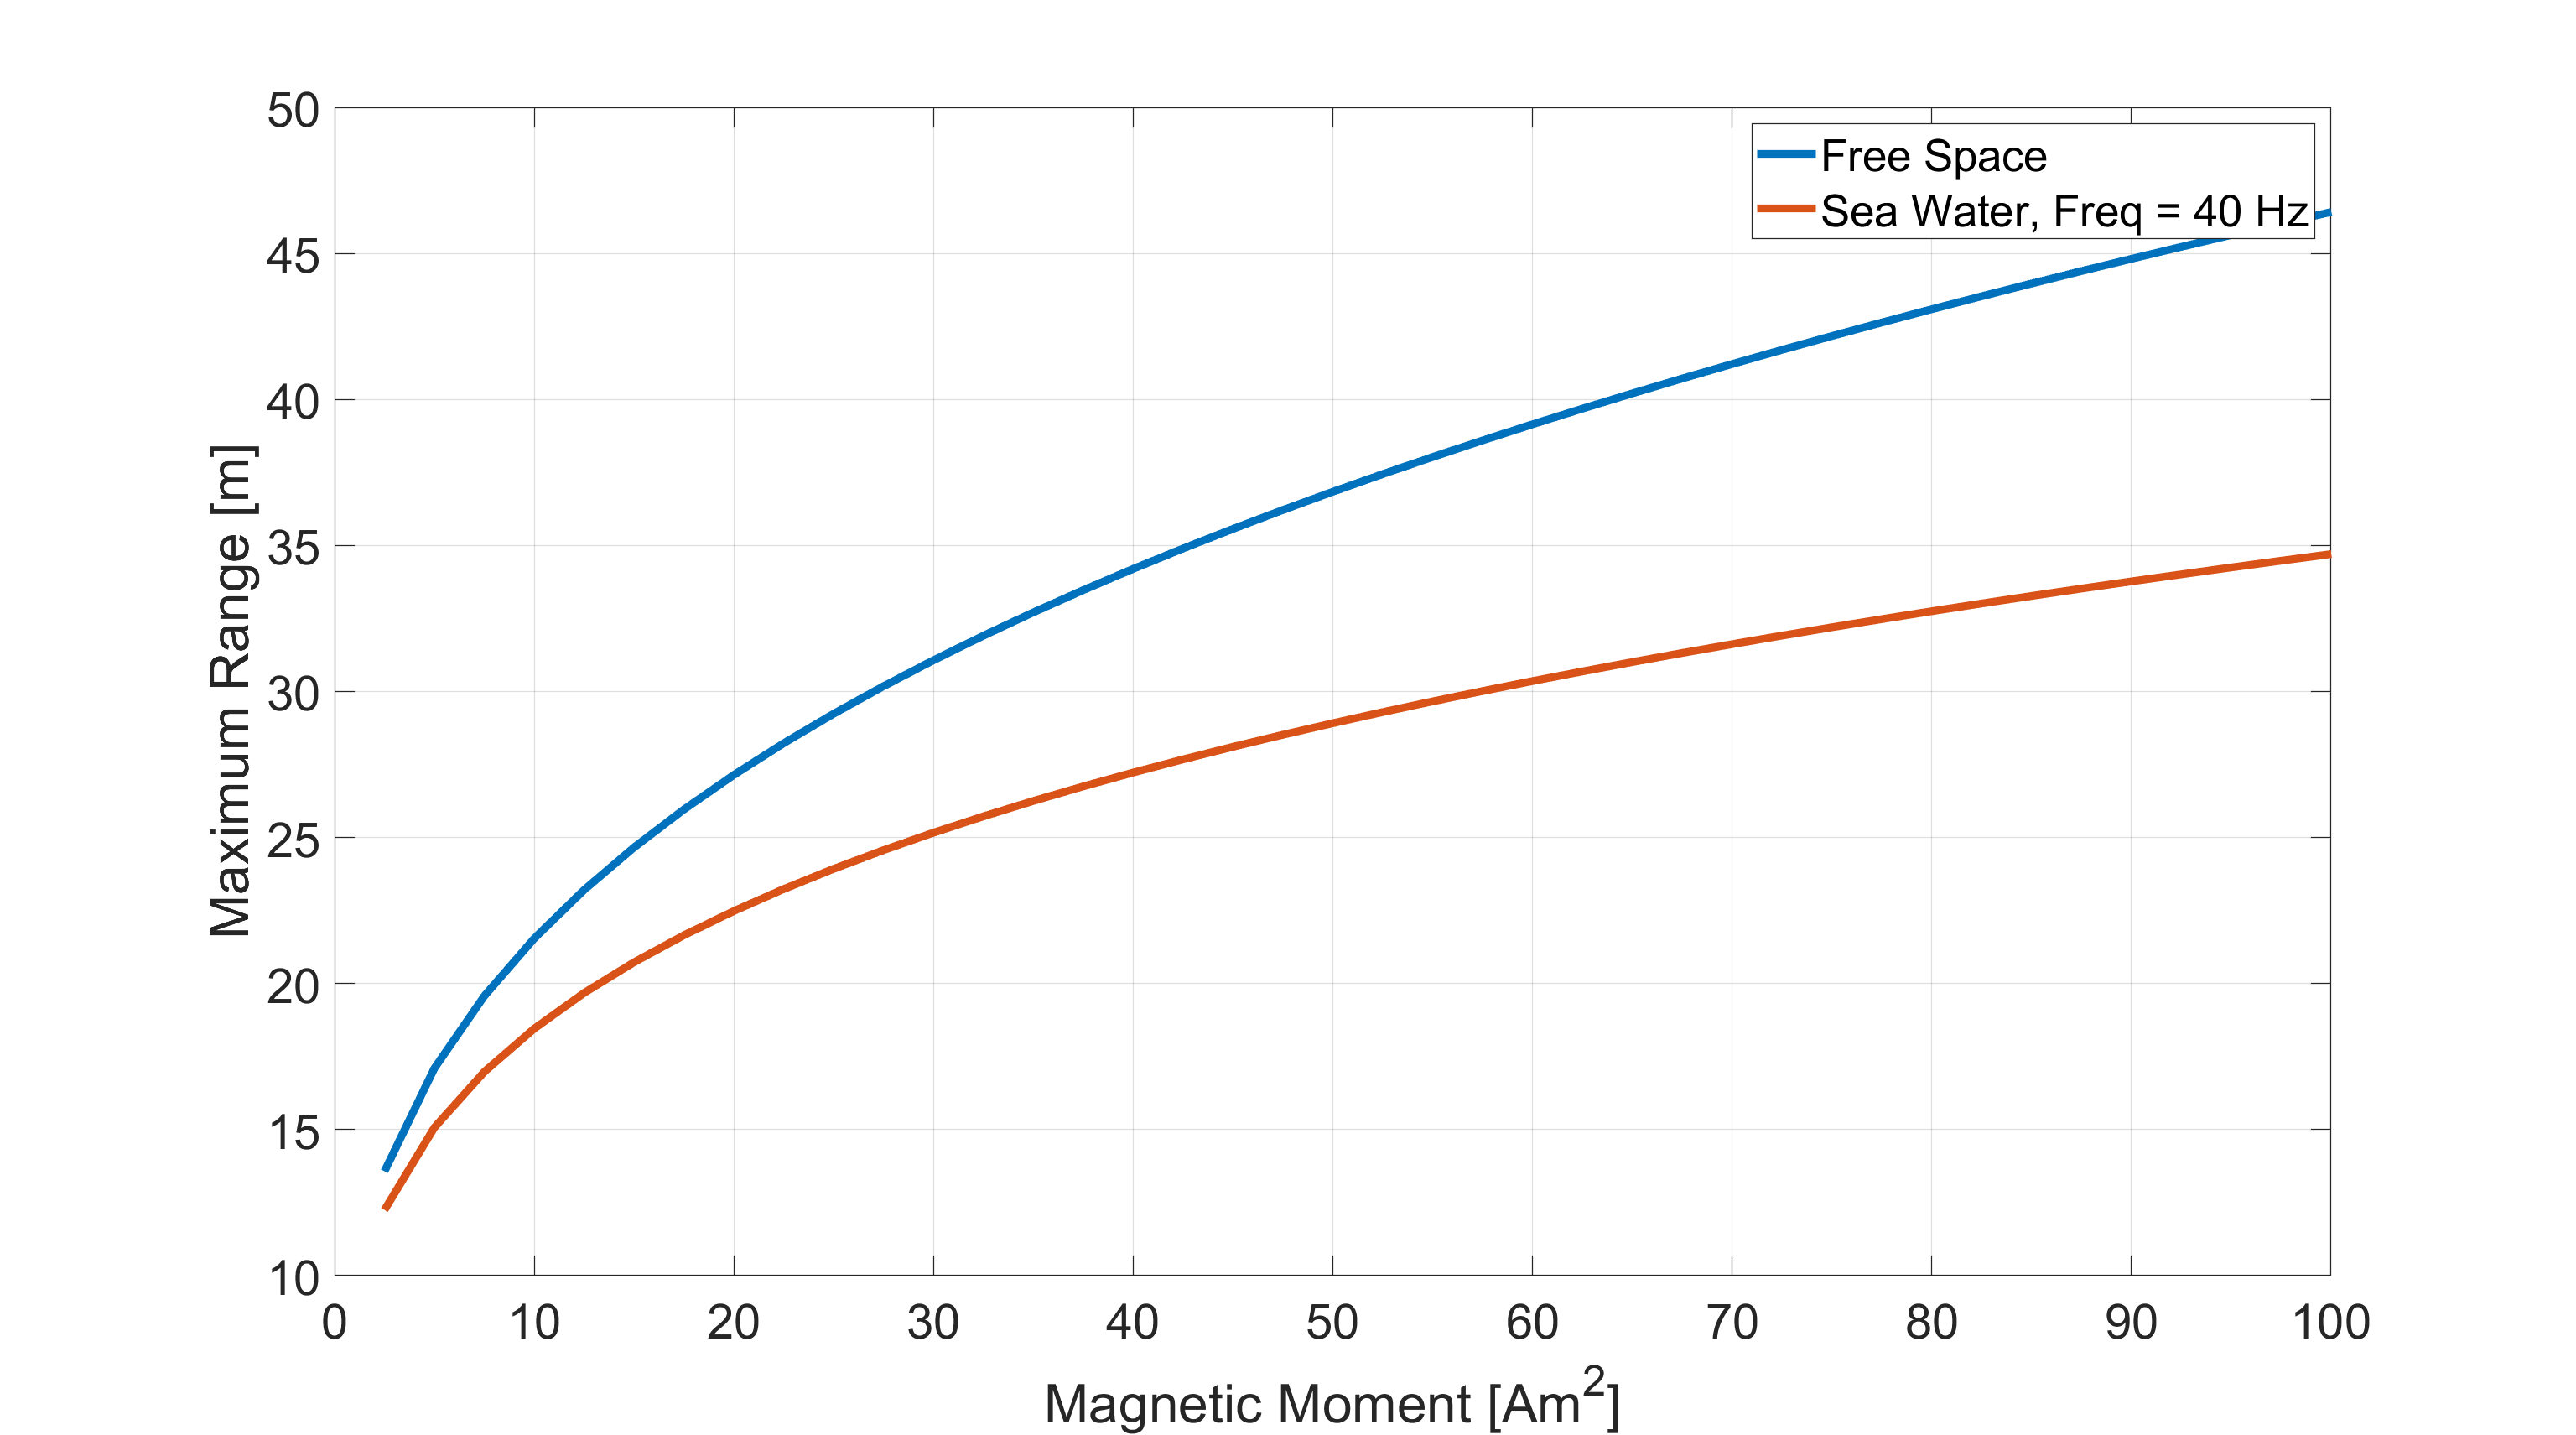
\includegraphics[width=0.8\textwidth]{Magnetic_Moment.png}
    \caption{Effective range of the coil in water.}
\label{fig:Effective Range}
\end{figure}
\subsection{iNav Configuration}

The SpeedyBee F405 V4 flight controller was flashed with iNav 7 firmware to enable GPS-based return-to-home (RTH) functionality and manual control. iNav 7 was selected because of its improved support for surface vehicles, enhanced GPS navigation features, and full compatibility with the SpeedyBee F405 V4 without requiring custom firmware builds.

\subsubsection*{Mixer Modifications}

By default, iNav's boat mixer uses differential thrust with two motors for steering. Since our ASV uses a single brushed DC motor for propulsion and a rudder servo for steering, this default configuration was unsuitable.

To support our hardware, we modified the mixer setup in \texttt{mixer.c} to map throttle directly to Motor 0 and yaw to Servo 0. Pitch and roll mixing were disabled, as they are unnecessary for surface operation. This allowed the boat to steer using the rudder while maintaining forward propulsion with the single motor.

\subsubsection*{Firmware Configuration Changes}

Several key settings were configured using the iNav Configurator and CLI to support manual control and GPS-assisted return-to-home:

\begin{itemize}
    \item \textbf{Ports:}
    \begin{itemize}
        \item UART6 configured for GPS (UBlox protocol)
        \item UART2 configured for SBUS receiver (FlySky FS-iA6B)
    \end{itemize}
    \item \textbf{Failsafe:} Configured to trigger Return-to-Home (RTH) on signal loss.
    \item \textbf{Flight Modes:} Enabled MANUAL, ANGLE, and RTH. AUTO mode was left disabled.
    \item \textbf{Arming:} Manual arming allowed when GPS lock is acquired.
    \item \textbf{PID Tuning:} Pitch and roll control disabled; yaw PID tuned for surface steering only.
\end{itemize}

Example CLI commands used:

\begin{lstlisting}
mixer load boat
set gps_provider = UBLOX
set gps_auto_config = ON
set gps_auto_baud = ON
set serialrx_provider = SBUS
set failsafe_procedure = RTH
set nav_rth_allow_landing = OFF
save
\end{lstlisting}

\subsubsection*{Source Code Adjustments}

The full iNav firmware was not rewritten, but minor modifications were made to the mixer definitions in \texttt{mixer.c} to support single-motor with rudder control. No other firmware files were changed. iNav’s official repository was used as the base.

\subsubsection*{Reproduction Instructions}

To reproduce this firmware setup:

\begin{enumerate}
    \item Clone the official iNav firmware repository:
    \begin{lstlisting}
git clone https://github.com/iNavFlight/inav.git
cd inav
    \end{lstlisting}

    
    \item Modify \texttt{src/main/mixer/mixer.c} to implement a single-motor and rudder mixer by:
    \begin{itemize}
        \item \textbf{Disable pitch and roll mixing} by setting these inputs to zero in the \texttt{mixTable()} function:
        \begin{lstlisting}[language=C]
            input[ROLL] = 0;
            input[PITCH] = 0;
        \end{lstlisting}

        \item \textbf{Map throttle to Motor 0 only} by replacing the motor loop with:
        \begin{lstlisting}[language=C]
            for (int i = 0; i < motorCount; i++) {
                if (i == 0) {
                    motor[i] = mixerThrottleCommand;
                } else {
                    motor[i] = motorZeroCommand;
                }
            }
        \end{lstlisting}

        \item \textbf{Map yaw to Servo 0} by ensuring yaw control is configured in the servo mixer or output settings, instead of applying yaw to the motor mixer.
    \end{itemize}


    \item Build the firmware following iNav's official build instructions.

    \item Flash the compiled firmware to the SpeedyBee F405 V4.

    \item Apply the CLI configuration listed above.

    \item Test GPS lock, receiver input, motor output, rudder control, and Return-to-Home functionality before deployment.
\end{enumerate}

\subsubsection*{Summary}

These modifications allowed the ASV to operate with stable manual control and GPS-assisted return-to-home, while disabling unnecessary flight-specific features.

\bigskip

The complete project repository, including design documentation, hardware details, software configuration, and source code references, is available at:

\begin{center}
\url{https://github.com/grgao/boat/tree/main/ECE%20455_Report}
\end{center}